\subsubsection{Asset}\label{sssc:asset}
The \textit{Asset} class is essential to the system, as it represents the real world assets that are to be managed. The class contains the asset's name, a description, an identifier to help identify the physical asset by for instance using a barcode scanner, and the database ID of the department it belongs to. The asset also inherits from the \textit{FieldContainer} class, which contains a list of fields on the object. The asset does not contain a list of tags, as the relation between asset and tag is a many to many relation (see \autoref{sc:function_component}) and is thus stored separately in the database. 
\par
Aside form these properties the model also contains a few methods for creating a hash code for the asset, compare the asset to another object, and deserializing the asset's fields from a JSON format. 

\begin{figure}[H]
    \centering
    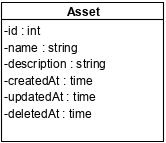
\includegraphics[width=0.25\textwidth]{figures/Classes/AssetAttributes.png}
    \caption{Asset class}
    \label{fig:AssetClass}
\end{figure}

\subsubsection{Tag}\label{sssc:tag}
The \textit{Tag} is one of the core components of the program. In the system these are defined by the interface \textit{ITagable} (see \autoref{code:ITagable}), which \textit{Tag} implements. This interface is implemented by the \textit{User} class as well, as both tag and user can be attached to assets. 
\par

\begin{listing}[H]
\begin{minted}[frame=lines, framesep=3mm, baselinestretch=1, linenos, bgcolor=LightGray, escapeinside='', breaklines]{csharp}

public interface ITagable
{
    ulong TagId { get; }
    Type TagType { get; }
    string TagLabel { get; }
    string FullTagLabel { get; set; }
    ulong ParentId { get; }
    int NumberOfChildren { get; }
    List<ITagable> Children { get; set; }
    string TagColor { get; set; }
    SolidColorBrush TagFontColor { get; }
}

\end{minted}
\captionof{listing}{The ITagable interface}
\label{code:ITagable}
\end{listing}

The \textit{Tag} class contains a \textit{Label}, \textit{Fields} and potentially a relation to a parent-tag by its ID. Parent tags are used to group tags, to make them easier to navigate and use (see \autoref{sc:model_component}). The relation between a parent and a child tag is a many to one relation stored on the child tag.
\par
Besides the properties inherited from \textit{Model}, the \textit{Tag} class also contains a \textit{FieldList} inherited from the \textit{FieldContainer}, a \textbf{Color}, and a \textit{DepartmentId}.
\par
The relation between an \textit{Asset} and a \textit{Tag} is defined in a relational database, containing the ID's of the connected tags and assets (see \autoref{sc:Tagging}).

\begin{figure}[H]
    \centering
    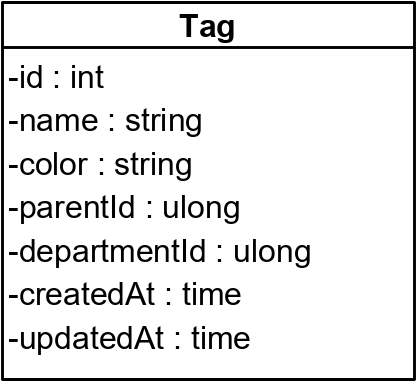
\includegraphics[width=0.25\textwidth]{figures/Implementation/Models/TagAttributes.png}
    \caption{Tag class}
    \label{fig:TagClass}
\end{figure}

% The diagram is purely illustrative, as the implementation of this relation is accomplished through a couple of attributes on the tag class. One of the attributes is called \textit{parentId} and contains the ID of the parent of the current tag. If the tag has no parent, this ID is 0. The other is called \textit{NumberOfChildren} and contains the number of tags attached to the current tag as its children.

\subsubsection{User} \label{sssc:Users}
Like the \textit{Tag} class, the \textit{User} class implements the interface \textit{ITagable} and mostly behaves like a \textit{Tag}.